\lab{Newton's Method}{Newton's Method}
\label{lab:NewtonsMethod}
\objective{Newton's method, the classical method for finding the zeros of a function, is one of the most important algorithms of all time.
In this lab we implement Newton's method in arbitrary dimensions and use it to solve a few interesting problems.
We also explore in some detail the convergence (or lack of convergence) of the method under various circumstances.}

\section*{Iterative Methods} % ================================================

An \emph{iterative method} is an algorithm that must be applied repeatedly to obtain a result.
The general idea behind any iterative method is to make an initial guess at the solution to a problem, apply a few easy computations to better approximate the solution, use that approximation as the new initial guess, and repeat until done.
More precisely, let $F$ be some function used to approximate the solution to a problem.
Starting with an initial guess of $x_0$, compute
\begin{equation}x_{k+1} = F(x_k)\label{eq:iter-summary}\end{equation}
for successive values of $k$ to generate a sequence $(x_k)_{k=0}^\infty$ that hopefully converges to the true solution.
If the terms of the sequence are vectors, they are denoted by $\x_k$.

In the best case, the iteration converges to the true solution $x$, written $\lim_{k\rightarrow\infty} x_k = x$ or $x_k\rightarrow x$.
In the worst case, the iteration continues forever without approaching the solution.
In practice, iterative methods require carefully chosen \emph{stopping criteria} to guarantee that the algorithm terminates at some point.
The general approach is to continue iterating until the difference between two consecutive approximations is sufficiently small, and to iterate no more than a specific number of times.
That is, choose a very small $\epsilon > 0$ and an integer $N\in\mathbb{N}$, and update the approximation using (\ref{eq:iter-summary}) until either
\begin{equation} % Stopping Criteria.
|x_k - x_{k-1}| < \epsilon
\qquad \text{or} \qquad
k > N.
\end{equation}

The choices for $\epsilon$ and $N$ are significant: a ``large'' $\epsilon$ (such as $10^{-6}$) produces a less accurate result than a ``small'' $\epsilon$ (such $10^{-16}$), but demands less computations; a small $N$ (10) also potentially lowers accuracy, but detects and halts nonconvergent iterations sooner than a large $N$ (10,000).
In code, $\epsilon$ and $N$ are often named \li{tol} and \li{maxiter}, respectively (or similar).

While there are many ways to structure the code for an iterative method, probably the cleanest way is to combine a \li{for} loop with a \li{break} statement.
As a very simple example, let $F(x) = \frac{x}{2}$.
This method converges to $x = 0$ independent of starting point.

\begin{lstlisting}
>>> F = lambda x: x / 2
>>> x0, tol, maxiter = 10, 1e-9, 8
>>> for k in range(maxiter):           # Iterate at most N times.
...     print(x0, end='  ')
...     x1 = F(x0)                      # Compute the next iteration.
...     if abs(x1 - x0) < tol:          # Check for convergence.
...         break                       # Upon convergence, stop iterating.
...     x0 = x1                         # Otherwise, continue iterating.
...
<<10  5.0  2.5  1.25  0.625  0.3125  0.15625  0.078125>>
\end{lstlisting}

In this example, the algorithm terminates after $N=8$ iterations (the maximum number of allowed iterations) because the tolerance condition $|x_k - x_{k-1}| < 10^{-9}$ is not met fast enough.
If $N$ had been larger (say $40$), the iteration would have quit early due to the tolerance condition.

\section*{Newton's Method in One Dimension} % =================================

\emph{Newton's method} is an iterative method for finding the zeros of a function.
That is, if $f:\mathbb{R}\rightarrow\mathbb{R}$, the method attempts to find a $\bar{x}$ such that $f(\bar{x}) = 0$.
Beginning with an initial guess $x_0$, calculate successive approximations for $\bar{x}$ with the recursive sequence
\begin{equation}
x_{k+1} = x_k - \frac{f(x_k)}{f'(x_k)}.
\label{eq:newton-1d-def}
\end{equation}

The sequence converges to the zero $\bar{x}$ of $f$ if three conditions hold:
\begin{enumerate}
\item $f$ and $f'$ exist and are continuous,
\item $f'(\bar{x})\neq0$, and
\item $x_0$ is ``sufficiently close'' to $\bar{x}$.
\end{enumerate}
In applications, the first two conditions usually hold.
If $\bar{x}$ and $x_0$ are not ``sufficiently close,'' Newton's method may converge very slowly, or it may not converge at all.
However, when all three conditions hold, Newton's method converges quadratically, meaning that the maximum error is squared at every iteration.
This is very quick convergence, making Newton's method as powerful as it is simple.

\begin{figure}[h] % Iterations of Newton's method.
\centering
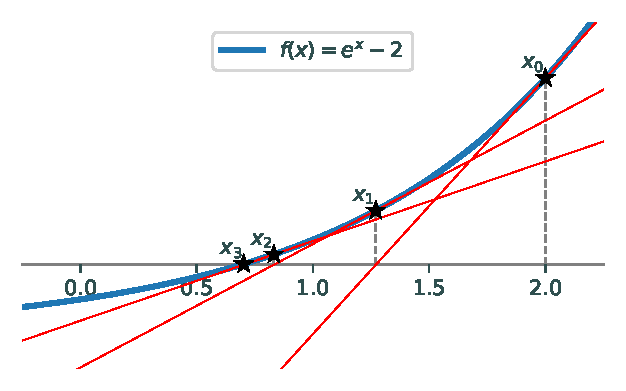
\includegraphics[width=.7\textwidth]{figures/newton_iters.pdf}
\caption{
Newton's method approximates the zero of a function (blue) by choosing as the next approximation the $x$-intercept of the tangent line (red) that goes through the point $(x_k, f(x_k))$.
In this example, $f(x) = e^x - 2$, which has a zero at $\bar{x} = \log(2)$.
Setting $x_0 = 2$ and using (\ref{eq:newton-1d-def}) to iterate, we have $x_1 = x_0 - \frac{f(x_0)}{f'(x_0)} = 2 - \frac{e^2 - 2}{e^2} \approx 1.2707$.
Similarly, $x_2 \approx 0.8320$, $x_3 \approx .7024$, and $x_4 \approx 0.6932$.
After only a few iterations, the zero $\log(2)\approx 0.6931$ is already computed to several digits of accuracy.}
\label{fig:newton}
\end{figure}

\begin{problem}
\label{prob:newton-basic}
Write a function that accepts a function $f$, an initial guess $x_0$, the derivative $f'$, a stopping tolerance defaulting to $10^{-5}$, and a maximum number of iterations defaulting to $15$.
Use Newton's method as described in (\ref{eq:newton-1d-def}) to compute a zero $\bar{x}$ of $f$.
Terminate the algorithm when $|x_k - x_{k-1}|$ is less than the stopping tolerance or after iterating the maximum number of allowed times.
Return the last computed approximation to $\bar{x}$, a boolean value indicating whether or not the algorithm converged, and the number of iterations completed.

Test your function against functions like $f(x) = e^x - 2$ (see Figure \ref{fig:newton}) or $f(x) = x^4 - 3$.
Check that the computed zero $\bar{x}$ satisfies $f(\bar{x}) \approx 0$.
Also consider comparing your function to \li{scipy.optimize.newton()}, which accepts similar arguments.
\end{problem}

\begin{info}
Newton's method can be used to find zeros of functions that are hard to solve for analytically.
For example, the function $f(x) = \frac{\sin(x)}{x}-x$ is not continuous on any interval containing 0, but it can be made continuous by defining $f(0)=1$.
Newton's method can then be used to compute the zeros of this function.
\end{info}

\begin{problem}{Application to interest rates}{}
\label{prob:newton-interest}
Suppose that an amount of $P_1$ dollars is put into an account at the beginning of years $1, 2,..., N_1$ and that the account accumulates interest at a fractional rate $r$ (so $r = .05$ corresponds to $5\%$ interest).
In addition, at the beginning of years $N_1 + 1, N_1 + 2, ..., N_1 + N_2$, an amount of $P_2$ dollars is withdrawn from the account and that the account balance is exactly zero after the withdrawal at year $N_1 + N_2$.
Then the variables satisfy
\[
P_1[(1+r)^{N_1} - 1] = P_2[1-(1+r)^{-N_2}].
\]

Write a function that, given $N_1$, $N_2$, $P_1$, and $P_2$, uses Newton's method to determine $r$.
For the initial guess, use $r_0 = 0.1$.
\\(Hint: Construct $f(r)$ such that when $f(r)=0$, the equation is satisfied.
Also compute $f'(r)$.)

To test your function, if $N_1 =30, N_2 =20, P_1 =2000$, and $P_2 =8000$, then $r\approx 0.03878$.
(From Atkinson, page 118). % TODO: better citation.
\end{problem}

\subsection*{Backtracking} % --------------------------------------------------

Newton's method may not converge for a variety of reasons.
One potential problem occurs when the step from $x_k$ to $x_{k+1}$ is so large that the zero is stepped over completely.
\emph{Backtracking} is a strategy that combats the problem of overstepping by moving only a fraction of the full step from $x_k$ to $x_{k+1}$.
This suggests a slight modification to (\ref{eq:newton-1d-def}),
\begin{equation}
x_{k+1} = x_k - \alpha\frac{f(x_k)}{f'(x_k)},\qquad\alpha\in(0,1].
\label{eq:newton-backtracking-1d}
\end{equation}
Note that setting $\alpha = 1$ results in the exact same method defined in (\ref{eq:newton-1d-def}), but for $\alpha \in (0,1)$, only a fraction of the step is taken at each iteration.

\begin{problem}{Implement backtracking}{}
Modify your function from Problem \ref{prob:newton-basic} so that it accepts a parameter $\alpha$ that defaults to $1$.
Incorporate (\ref{eq:newton-backtracking-1d}) to allow for backtracking.

To test your modified function, consider $f(x)=x^{1/3}$.
The command \li{x**(1/3.)} fails when \li{x} is negative, so the function can be defined with NumPy as follows.
\begin{lstlisting}
import numpy as np
f = lambda x: np.sign(x) * np.power(np.<<abs>>(x), 1./3)
\end{lstlisting}
With $x_0=.01$ and $\alpha=1$, the iteration should \textbf{not} converge.
However, setting $\alpha=.4$, the iteration should converge to a zero that is close to $0$.
\label{prob:newton-1d-backtracking}
\end{problem}

The backtracking constant $\alpha$ is significant, as it can result in faster convergence or convergence to a different zero (see Figure \ref{fig:newton-backtracking-multi-result}).
However, it is not immediately obvious how to choose an optimal value for $\alpha$.

\begin{figure}[H]
\centering
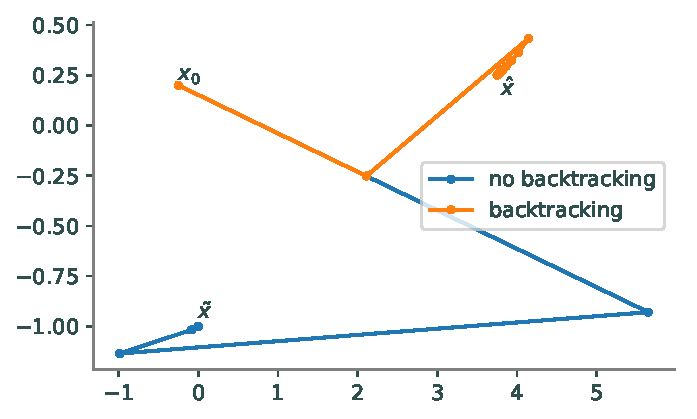
\includegraphics[width=.7\textwidth]{figures/backtracking.pdf}
\caption{Starting at the same initial value but using different backtracking constants can result in convergence to two different solutions.
The blue line converges to $\tilde{\x} = (0,-1)$ with $\alpha = 1$ in 5 iterations of Newton's method while the orange line converges to $\hat{\x} = (3.75,.25)$ with $\alpha = 0.4$ in $15$ iterations.
Note that the points in this example are $2$-dimensional, which is discussed in the next section.}
\label{fig:newton-backtracking-multi-result}
\end{figure}

\begin{problem}{Searching for a good backtracking constant}{}
\label{prob:newton-backtracking-search}
Write a function that accepts the same arguments as your function from Problem \ref{prob:newton-1d-backtracking} except for $\alpha$.
Use Newton's method to find a zero of $f$ using various values of $\alpha$ in the interval $(0,1]$.
Plot the values of $\alpha$ against the number of iterations performed by Newton's method.
Return a value for $\alpha$ that results in the lowest number of iterations.

A good test case for this problem is the function $f(x) = x^{1/3}$ discussed in Problem \ref{prob:newton-1d-backtracking}.
In this case, your plot should show that the optimal value for $\alpha$ is actually closer to $.3$ than to $.4$.
% resemble the following figure.
% \begin{figure}[H]
% \includegraphics[width=.7\textwidth]{figures/alpha_iters.pdf}
% \end{figure}
\end{problem}

\section*{Newton's Method in Higher Dimensions} % =============================

Newton's method can be generalized to work on functions with a multivariate domain and range.
Let $f:\mathbb{R}^n\rightarrow\mathbb{R}^n$ be given by $f(\x)=[f_1(\x)\ f_2(\x)\ \ldots\ f_k(\x)]\trp$, with $f_i:\mathbb{R}^n\to\mathbb{R}$ for each $i$.
The derivative $Df:\mathbb{R}^n\rightarrow\mathbb{R}^{n\times n}$ is the $n\times n$ Jacobian matrix of $f$.
\[
Df =
\left[\begin{array}{ccc}
\frac{\partial f_1}{\partial x_1} & \cdots & \frac{\partial f_1}{\partial x_k} \\
\vdots & \ddots & \vdots \\
\frac{\partial f_n}{\partial x_1} & \cdots & \frac{\partial f_n}{\partial x_k} \\
\end{array}\right]
\]

In this setting, Newton's method seeks a vector $\bar{\x}$ such that $f(\bar{\x}) = \0$, the vector of $n$ zeros.
With backtracking incorporated, (\ref{eq:newton-backtracking-1d}) becomes
\begin{equation}
\x_{k+1} = \x_k - \alpha{Df(\x_k)}^{-1}{f(\x_k)}.
\label{eq:newton-nd}
\end{equation}
Note that if $n = 1$, (\ref{eq:newton-nd}) is exactly (\ref{eq:newton-backtracking-1d}) because in that case, $Df(x)^{-1} = 1/f'(x)$.

This vector version of Newton's method terminates when the maximum number of iterations is reached or the difference between successive approximations is less than a predetermined tolerance $\epsilon$ with respect to a vector norm, that is, $||\x_k - \x_{k-1}|| < \epsilon$.

\begin{problem}{Newton's method in n dimensions}{}
Modify your function from Problems \ref{prob:newton-basic} and \ref{prob:newton-1d-backtracking} so that it can compute a zero of a function $f:\mathbb{R}^n\rightarrow\mathbb{R}^n$ for any $n\in\mathbb{N}$.
Take the following tips into consideration.
\begin{itemize}
\item If $n > 1$, $f$ should be a function that accepts a 1-D NumPy array with $n$ entries and returns another NumPy array with $n$ entries.
Similarly, $Df$ should be a function that accepts a 1-D array with $n$ entries and returns a $n\times n$ array.
In other words, $f$ and $Df$ are callable functions, but $f(\x)$ is a vector and $Df(\x)$ is a matrix.

\item \li{np.isscalar()} may be useful for determining whether or not $n > 1$.

\item Instead of computing $Df(\x_k)^{-1}$ directly at each step, solve the system $Df(\x_k)\y_k = f(\x_k)$ and set $\x_{k+1} = \x_k - \alpha\y_k$.
In other words, use \li{la.solve()} instead of \li{la.inv()}.
% Always avoid taking matrix inverses when possible.

\item The stopping criterion now requires using a norm function instead of \li{abs()}.
\end{itemize}

After your modifications, carefully verify that your function still works in the case that $n=1$, and that your functions from Problems \ref{prob:newton-interest} and \ref{prob:newton-backtracking-search} also still work correctly.
In addition, your function from Problem \ref{prob:newton-backtracking-search} should also work for any $n \in \mathbb{N}$.
\label{prob:newton-nd-implementation}
\end{problem}

\begin{problem}{Bioremediation}{}
Bioremediation involves the use of bacteria to consume toxic wastes.
At a steady state, the bacterial density $x$ and the nutrient concentration $y$ satisfy the system of nonlinear equations
\begin{align*}
\gamma xy - x(1 + y) &= 0 \\
-xy + (\delta - y)(1 + y) &= 0,
\end{align*}
where $\gamma$ and $\delta$ are parameters that depend on various physical features of the system.%
\footnote{This problem is adapted from exercise 5.19 of \cite{heath2002scientific} and the notes of Homer Walker).}

For this problem, assume the typical values $\gamma = 5$ and $\delta = 1$, for which the system has solutions at $(x, y) = (0, 1), (0, -1)$, and $(3.75, .25)$.
Write a function that finds an initial point $\x_0 = (x_0,y_0)$ such that Newton's method converges to either $(0, 1)$ or $(0, -1)$ with $\alpha = 1$, and to $(3.75, .25)$ with $\alpha = 0.55$.
As soon as a valid $\x_0$ is found, return it (stop searching).
\\(Hint: search within the rectangle $[-\frac{1}{4},0]\times[0,\frac{1}{4}]$.)
\end{problem}

\subsection*{Basins of Attraction} % ------------------------------------------

When a function $f$ has many zeros, the zero that Newton's method converges to depends on the initial guess $x_0$.
For example, the function $f(x)=x^2-1$ has zeros at $-1$ and $1$.
If $x_0<0$, then Newton's method converges to $-1$; if $x_0 > 0$ then it converges to $1$ (see Figure \ref{fig:basins-quadratic}).
The regions $(-\infty, 0)$ and $(0, \infty)$ are called the \emph{basins of attraction} of $f$.
Starting in one basin of attraction leads to finding one zero, while starting in another basin yields a different zero.

When $f$ is a polynomial of degree greater than 2, the basins of attraction are much more interesting.
For example, the basis of attraction for $f(x) = x^3-x$ are shown in Figure \ref{fig:basins-cubic}.
The basin for the zero at the origin is connected, but the other two basins are disconnected and share a kind of symmetry.

\begin{figure}[H] % 1-D basins of attraction.
\centering
\begin{subfigure}{.48\textwidth}
    \centering
    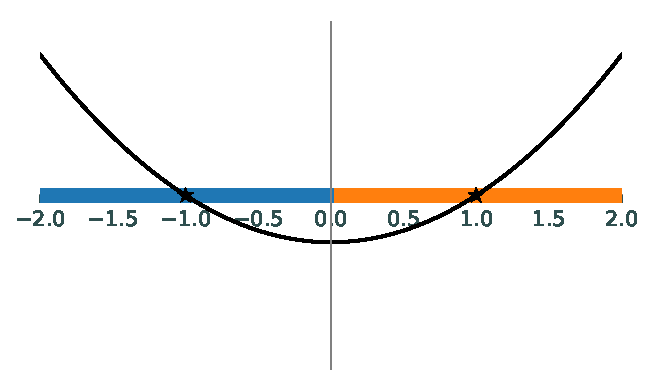
\includegraphics[width=\textwidth]{figures/basins_quadratic.pdf}
    \caption{Basins of attraction for $f(x) = x^2 -1$.}
    % With $\alpha=1$, blue values for $x_0$ converge to -1 and orange values converge to 1.}
    \label{fig:basins-quadratic}
\end{subfigure}
\quad
\begin{subfigure}{.48\textwidth}
    \centering
    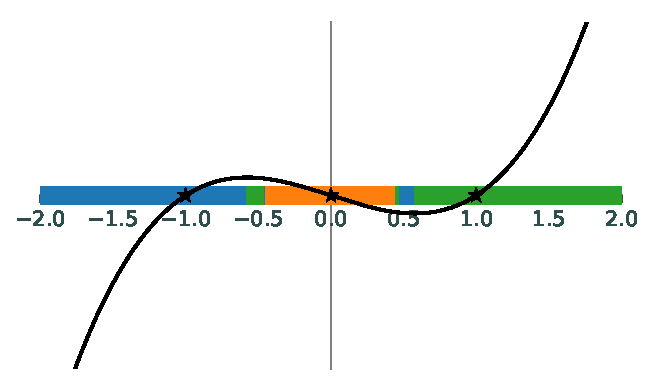
\includegraphics[width=\textwidth]{figures/basins_cubic.pdf}
    \caption{Basins of attraction for $f(x) = x^3 -x$.}
        % With $\alpha=1$, blue values converge to $-1$, orange converge to 0, and green converge to 1.}
    \label{fig:basins-cubic}
\end{subfigure}
\caption{Basins of attraction with $\alpha=1$.
Since choosing a different value for $\alpha$ can change which zero Newton's method converges to, the basins of attraction may change for other values of $\alpha$.}
\end{figure}

It can be shown that Newton's method converges in any Banach space with only slightly stronger hypotheses than those discussed previously. % \footnote{See Chapter 7 of Volume 1 for details.}
In particular, Newton's method can be performed over the complex plane $\mathbb{C}$ to find imaginary zeros of functions.
Plotting the basins of attraction over $\mathbb{C}$ yields some interesting results.

The zeros of $f(x) = x^3 - 1$ are $1$, and $-\frac{1}{2} \pm \frac{\sqrt{3}}{2}i$.
To plot the basins of attraction for $f(x) = x^3-1$ on the square complex domain $X = \{a+bi \mid a \in [-\frac{3}{2},\frac{3}{2}], b \in [-\frac{3}{2},\frac{3}{2}]\}$,
create an initial grid of complex points in this domain using \li{np.meshgrid()}.
% Create the real and imaginary parts of the points separately, and then use \li{np.meshgrid()} to turn them into a single grid of complex numbers.

\begin{lstlisting}
>>> x_real = np.linspace(-1.5, 1.5, 500)    # Real parts.
>>> x_imag = np.linspace(-1.5, 1.5, 500)    # Imaginary parts.
>>> X_real, X_imag = np.meshgrid(x_real, x_imag)
>>> X_0 = X_real + 1j*X_imag                # Combine real and imaginary parts.
\end{lstlisting}

The grid $X_0$ is a $500\times500$ array of complex values to use as initial points for Newton's method.
Array broadcasting makes it easy to compute an iteration of Newton's method at every grid point.

\begin{lstlisting}
>>> f = lambda x: x**3 - 1
>>> Df = lambda x: 3*x**2
>>> X_1 = X_0 - f(X_0)/Df(X_0)
\end{lstlisting}

After enough iterations, the $(i,j)$th element of the grid $X_k$ corresponds to the zero of $f$ that results from using the $(i,j)$th element of $X_0$ as the initial point.
For example, with $f(x) = x^3 - 1$, each entry of $X_k$ should be close to $1$, $-\frac{1}{2} + \frac{\sqrt{3}}{2}i$, or $-\frac{1}{2} - \frac{\sqrt{3}}{2}i$.
Each entry of $X_k$ can then be assigned a value indicating which zero it corresponds to.
Some results of this process are displayed below.

\begin{figure}[H]
\centering
\begin{subfigure}{.49\textwidth}
    \centering
    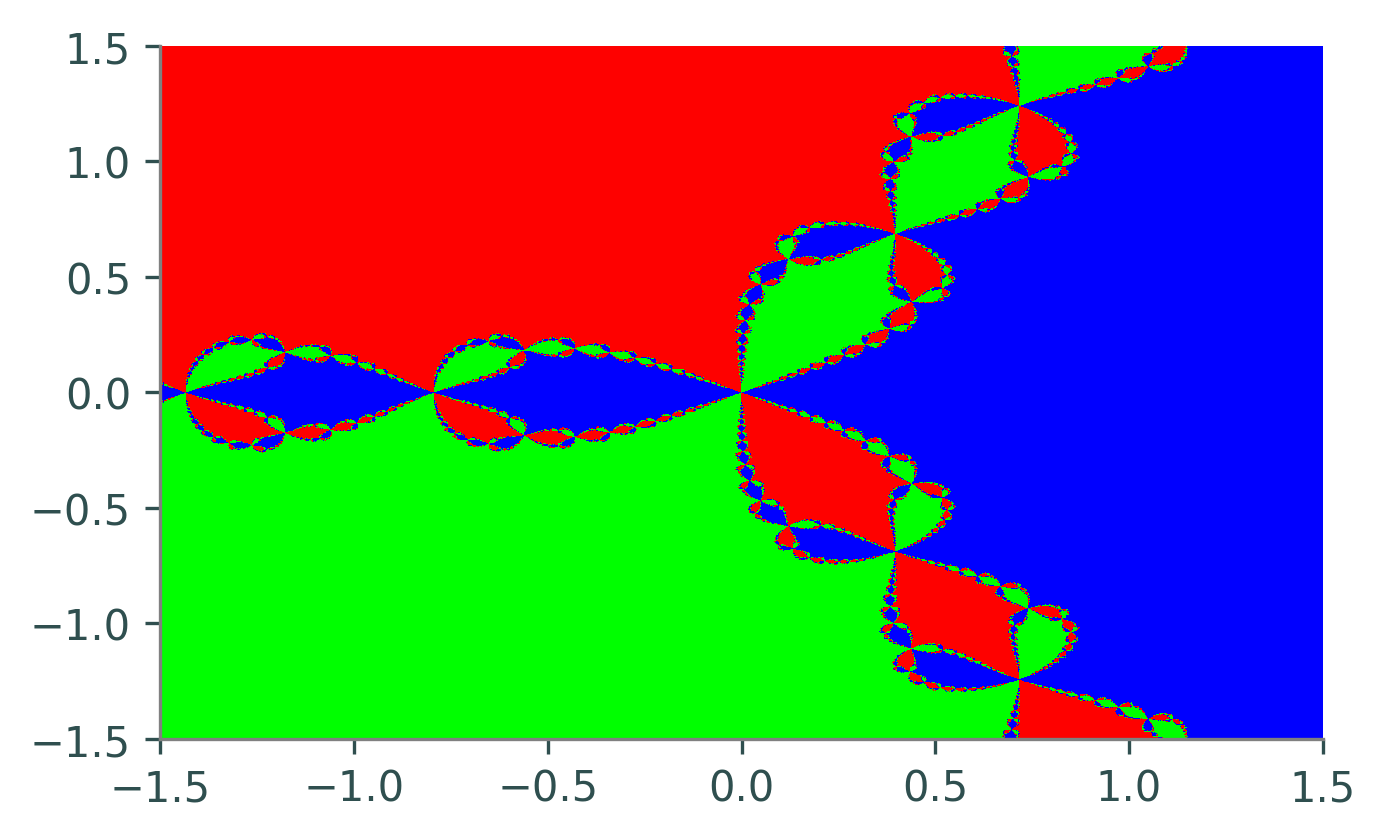
\includegraphics[width=\textwidth]{figures/fractal_hw.png}
    \caption{Basins of attraction for $f(x) = x^3-1$.}
    \label{fig:fractal_hw}
\end{subfigure}
\begin{subfigure}{.49\textwidth}
    \centering
    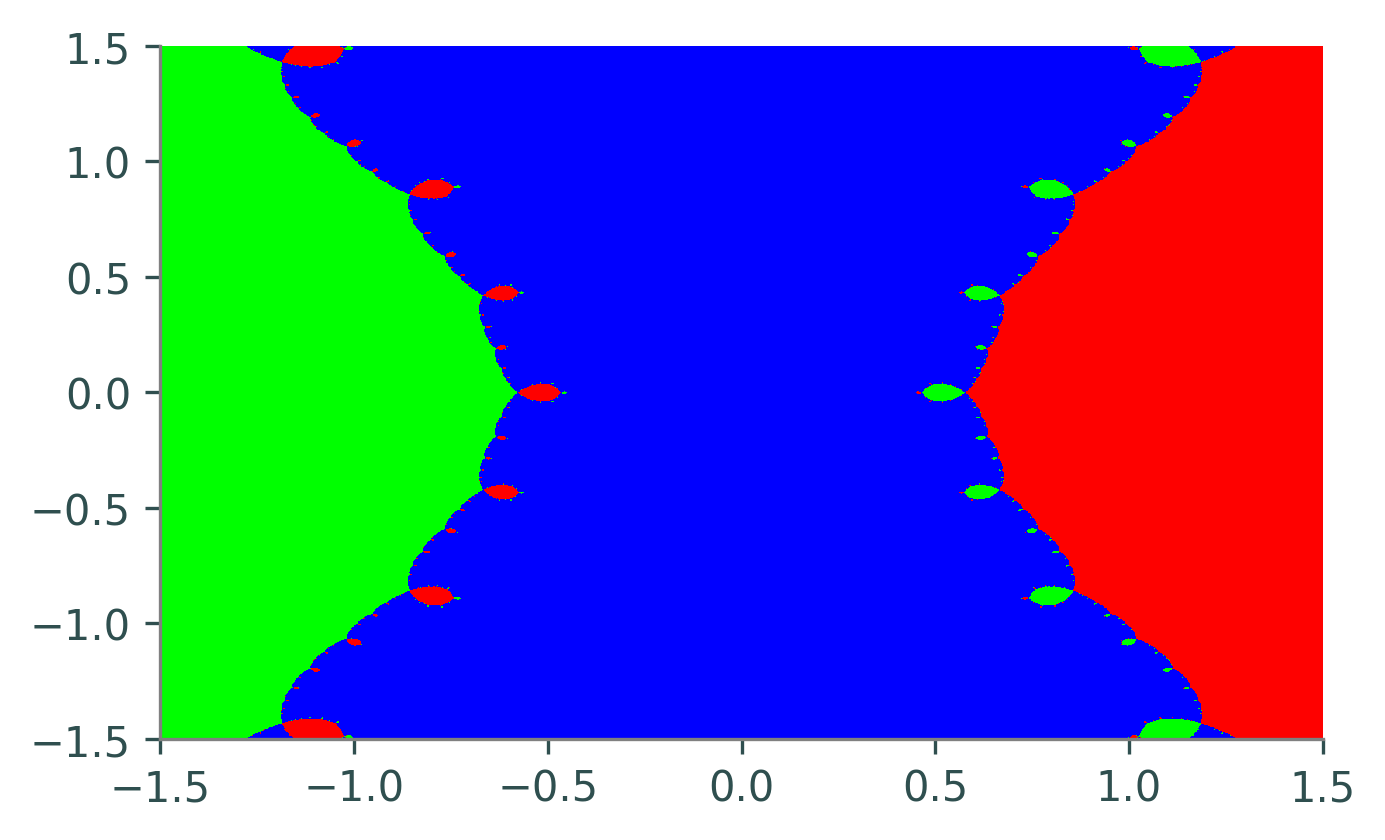
\includegraphics[width=\textwidth]{figures/fractal_ex.png}
    \caption{Basins of attraction for $f(x) = x^3-x$.}
    \label{fig:fractal_ex}
\end{subfigure}
\caption{}
\label{fig:newton-basins}
\end{figure}

\begin{info} % Newton fractals
Notice that in some portions of Figure \ref{fig:fractal_hw}, whenever red and blue try to come together, a patch of green appears in between.
This behavior repeats on an infinitely small scale, producing a fractal.
Because it arises from Newton's method, this kind of fractal is called a \emph{Newton fractal}.

Newton fractals show that the long-term behavior of Newton's method is \textbf{extremely} sensitive to the initial guess $x_0$.
Changing $x_0$ by a small amount can change the output of Newton's method in a seemingly random way.
This phenomenon is called \emph{chaos} in mathematics.
\end{info}

\begin{problem}{Plot the basins of attraction}{}
Write a function that accepts a function $f\colon\mathbb{C}\rightarrow\mathbb{C}$, its derivative $f'\colon\mathbb{C}\rightarrow\mathbb{C}$, an array \li{zeros} of the zeros of $f$, bounds $[r_{\text{min}},r_{\text{max}},i_{\text{min}},i_{\text{max}}]$ for the domain of the plot, an integer \li{res} that determines the resolution of the plot, and number of iterations \li{iters} to run the iteration.
Compute and plot the basins of attraction of $f$ in the complex plane over the specified domain in the following steps.
\begin{enumerate}
\item Construct a \li{res}$\times$\li{res} grid $X_0$ over the domain $\{a+bi \mid a \in [r_{\text{min}},r_{\text{max}}], b \in [i_{\text{min}},i_{\text{max}}]\}$.

\item Run Newton's method (without backtracking) on $X_0$ \li{iters} times, obtaining the \li{res}$\times$\li{res} array $x_{k}$.
To avoid the additional computation of checking for convergence at each step, do not use your function from Problem \ref{prob:newton-nd-implementation}.

\item $X_k$ cannot be directly visualized directly because its values are complex.
Solve this issue by creating another \li{res}$\times$\li{res} array $Y$.
To compute the $(i,j)$th entry $Y_{i,j}$, determine which zero of $f$ is closest to the $(i,j)$th entry of $X_k$.
Set $Y_{i,j}$ to the index of this zero in the array \li{zeros}.
If there are $R$ distinct zeros, each $Y_{i,j}$ should be one of $0,1,\ldots,R-1$.
\\(Hint: \li{np.argmin()} may be useful.)

\item Use \li{plt.pcolormesh()} to visualize the basins.
Recall that this function accepts three array arguments: the $x$-coordinates (in this case, the real components of the initial grid), the $y$-coordinates (the imaginary components of the grid), and an array indicating color values ($Y$).
Set \li{cmap="brg"} to get the same color scheme as in Figure \ref{fig:newton-basins}.
\end{enumerate}

Test your function using $f(x) = x^3-1$ and $f(x)=x^3-x$.
The resulting plots should resemble Figures \ref{fig:fractal_hw} and \ref{fig:fractal_ex}, respectively (perhaps with the colors permuted).
\end{problem}

\begin{comment} % No Additional Material for now.

\newpage

\section*{Additional Material} % ==============================================

\subsection*{Newton's Method for Optimization} % ------------------------------

\subsection*{Other Algorithms Based on Newton's Method} % ---------------------

% \subsection*{Fractals} % ----------------------------------------------------

% % Totally irrelevant.
% Another well-studied fractal in the complex plane is the Mandelbrot set.
% It is defined as the points $c \in \mathbb{C}$ for which the sequence
% \[z_k = z_{k-1}^2 + c\]
% is bounded.

\subsection*{Visualizing Complex Functions} % ---------------------------------

Plot the result of \li{np.angle()} on $X_k$ as an alternative to the index assignment.

\end{comment}
